\documentclass{standalone}
\usepackage{standalone}

\begin{document}
\subsection{Image Enhancement}
We modified the enhancement techniques described in \cite{Abolghasemi2009} and \cite{zheng2005efficient} followed by \cite{joarder2012bangla}. We used the Gaussian image to increase the contrast of the image around plate like regions. The formula used is shown in Equation \ref{eq:Enhancement}.

\begin{equation} \label{eq:Enhancement}
I' = f(\rho W_g) (I - \bar{I}) + \bar{I}
\end{equation}

In the equation \ref{eq:Enhancement},\\
$\bar{I}$ = the mean intensity. \\
$I$ = the intensity of the original image. \\
$I'$ = the new enhanced image. \\
$W_g$ = normalized Gaussian image. \\ 
$\rho W$ = the standard deviation of Gaussian image, and \\
$f$ = the weighting function defined in Equation \ref{eq:WeightFunction}.
\begin{equation} \label{eq:WeightFunction}
f(\rho W_g) = 
\begin{cases} 
	\dfrac{3}{ \dfrac{2}{0.3^2} ( \rho W_g - 0.3)^2 + 1 },
    	& \mbox{if } 0 \leq \rho W_g < 0.3  
     \\
    
    \dfrac{3}{ \dfrac{2}{(0.5 - 0.3)^2} ( \rho W_g - 0.3)^2 + 1 },
    	& \mbox{if } 0.3 \leq \rho W_g < 0.5  
     \\
        
    1	& \mbox{if } \rho W_g \geq 0
\end{cases}
\end{equation} 

Figure \ref{fig:WeightDistribution} shows the map of weight function from \ref{eq:WeightFunction}.
\begin{figure}
	\centering
	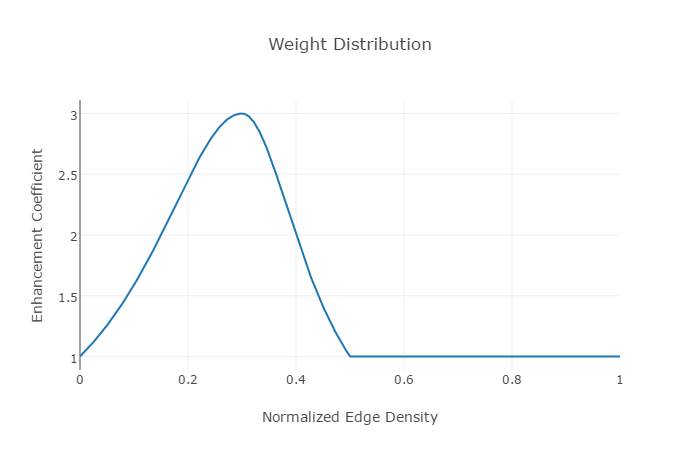
\includegraphics[width=.8\linewidth]{./img/plots/weight.png}
	\caption{Weight function against normalized edge density} 
	\label{fig:WeightDistribution}
\end{figure}

To increase the efficiency of the calculation the entire image is divided into $8 \times 8$ windows each having the size of $60 \times 80$. For each window we calculated weight and mean intensity using {\it Bilinear interpolation}. Also by using {\it numpy} library for matrix manipulation, we could dramatically decrease processing time.

Figure \ref{fig:EnhanceSample} shows the resulting image. The brightness of license plate area has significantly improved.
\begin{figure}
	\centering
	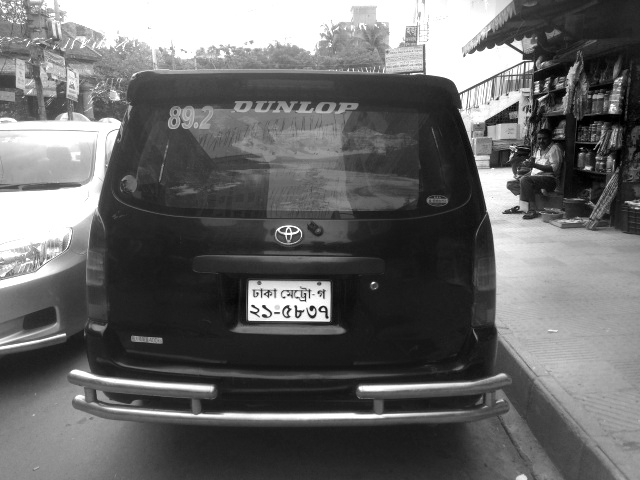
\includegraphics[width=.8\linewidth]{./img/sample/stage4.jpg}
	\caption{Enhanced Image} 
	\label{fig:EnhanceSample}
\end{figure}

\end{document}